\clearpage
\section{Sacred Vessels and Communion Vessels}
Among all sanctuary appointments, sacred vessels receive special honor because they hold the Body and Blood of Christ (GIRM 327). Universal law prescribes precious metal gilded inside where necessary, while United States adaptations permit solid, non-breaking, non-absorbent noble materials for patens, ciboria, and pyxes---never glass, earthenware, or clay, and never flagons for holding or pouring the consecrated Precious Blood.

\PCDPlateHeader{Plate III --- Sacred Vessels and Vessels for Communion}{Not to common scale}
\ifdefined\TriptychPrintEdition
\begin{center}
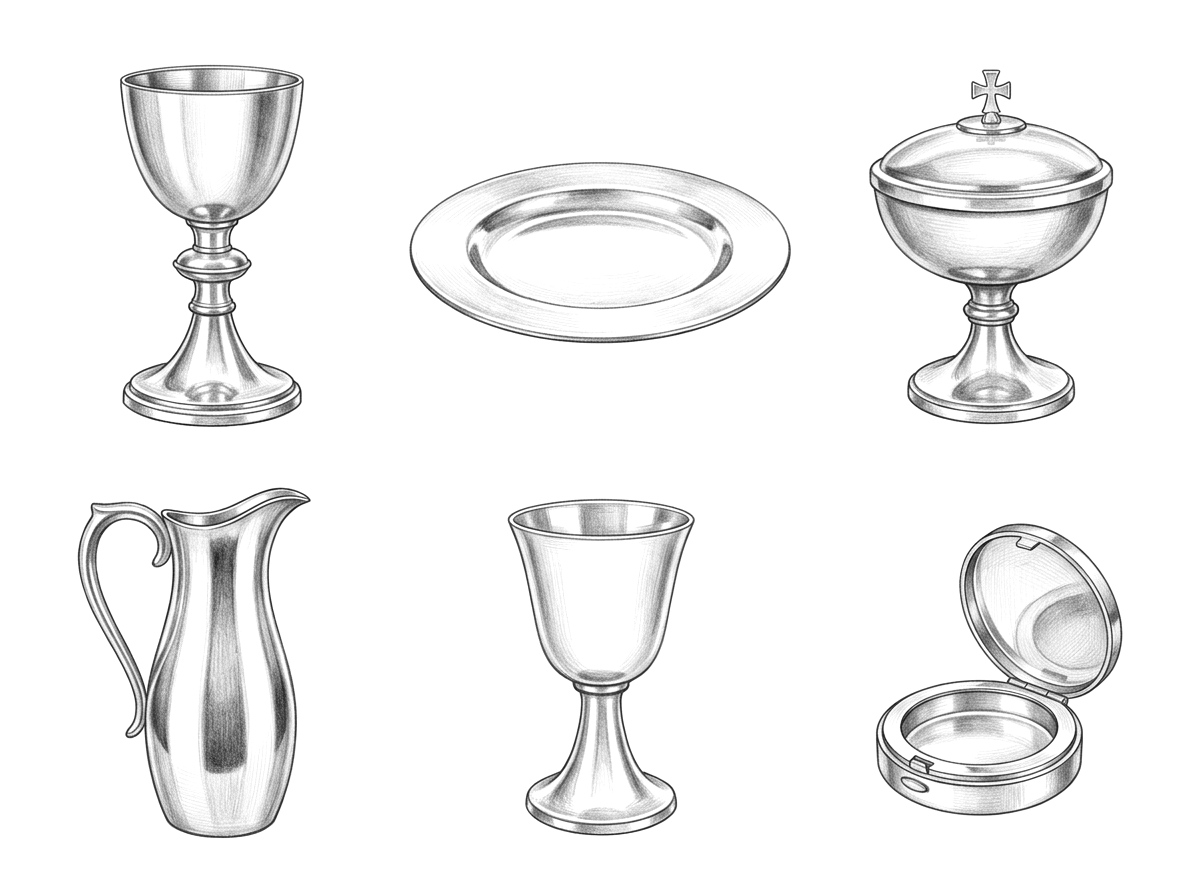
\includegraphics[width=0.92\linewidth,height=3.55in,keepaspectratio]{liturgy/roman-rite/postconciliar/2008-latin-2011-us-english/reference/roman-sanctuary-dictionary/shared/artwork/graphite/pc-art-03-sacred-vessels.png}
\end{center}
\PCDPositionKey{Top row, left to right: Chalice, wide shallow Paten, lidded footed Ciborium with cross finial. Bottom row, left to right: pitcher-style wine Flagon (pre-consecration transport only), footed Communion Cup (chalice), hinged pocket Pyx shown open.}
\else
\textbf{Visual Plate Summary (Plate III --- Sacred Vessels and Vessels for Communion, Not to common scale):} Six-vessel monochrome graphite comparison rendered with metallic reflections on white ground: top row left to right, a classical footed chalice with node, a broad shallow paten dish, and a lidded footed ciborium topped by a small cross; bottom row left to right, a tall slender pitcher-style wine flagon for bringing unconsecrated wine, a simpler footed Communion cup for distributing the Precious Blood, and a small hinged circular pocket pyx open to show its smooth gilded cavity.

\textbf{Reading order and object placement:} Top row, left to right: Chalice, wide shallow Paten, lidded footed Ciborium with cross finial. Bottom row, left to right: pitcher-style wine Flagon (pre-consecration transport only), footed Communion Cup (chalice), hinged pocket Pyx shown open.
\fi

\label{pc-obj-chalice}
\PCDEntryHead{Chalice}{Calix}{required}{N08}
\PCDField{Also called}{Principal Chalice; Eucharistic Chalice; \textit{Calix principalis}}
The chalice is the principal footed sacred vessel in which wine mingled with a drop of water is offered, consecrated into the Precious Blood of Christ, elevated in adoration, and consumed at Mass. Shown at top left of Plate III with a deep, smooth flared cup, a baluster stem bearing a central grip node (nodus) for steady elevation, and a broad weighted circular foot; Plate X shows it standing at the center of the unfolded corporal alongside the paten, veiled ciborium, and Communion cups.

\PCDField{Plate position and status}{Top left (Plate III); center of the unfolded corporal (Plate X) (Universal Roman law)}
\PCDField{Placement and liturgical use}{Before Mass with a congregation, the chalice stands prepared on the credence table with the corporal, purificator, optional pall, and---as a praiseworthy practice commended in GIRM 118c---covered with a chalice veil of the color of the day or white (GIRM 118c). At the Preparation of the Gifts, the deacon, instituted acolyte, or server brings it to the altar, where the priest or deacon pours wine and a little water into it (GIRM 139, 142, 178). After the consecration, the priest elevates the chalice and the deacon elevates it during the final doxology (GIRM 150--151, 180). Following Communion, any remaining Precious Blood is consumed reverently at the altar and the chalice is purified strictly by the priest, deacon, or instituted acolyte---never poured into the sacrarium or ground (GIRM 279; RS 119; USCCB Norms 52--55). Every chalice is blessed before liturgical use according to the Roman Ritual, praiseworthily by the diocesan bishop or by a priest (GIRM 333; RS 118).}
\PCDField{United States norm}{While USCCB GIRM 329 permits solid, noble, non-breaking, non-absorbent materials such as hard woods for patens, ciboria, and pyxes, universal law requires the chalice bowl to be completely nonabsorbent (GIRM 330) and precious metal gilded inside if the metal rusts or is less precious than gold (GIRM 328); glass, earthenware, and clay chalices are strictly reprobated (Redemptionis Sacramentum 117).}
\PCDField{Ministers and server boundary}{Ordinary ministers: Bishop, Priest, Deacon. Server prepares or sets in place before or during Mass: Servers may place the empty, unconsecrated chalice on the credence table before Mass and carry it to the altar at the Preparation of the Gifts if no deacon or instituted acolyte serves (GIRM 139). After consecration, servers never touch a chalice holding the Precious Blood, never consume from it, and never purify it (GIRM 279; RS 119; USCCB Norms 53).}
\PCDSafety{Once consecrated, the chalice contains the Blood of Christ: servers and extraordinary ministers never purify it (strictly reserved to priest, deacon, or instituted acolyte), and remaining Precious Blood is never poured into the sacrarium or onto the ground (USCCB Norms 53--55).}
\PCDField{Distinguish from}{Communion Cup, Ciborium, Flagon}
\PCDField{Symbolism}{The chalice bears singular honor as the cup of the New Covenant, recalling the Lord's words at the Last Supper in Matt 26:27--28 (``Drink ye all of this. For this is my blood of the new testament, which shall be shed for many unto remission of sins.''), St. Paul in 1 Cor 10:16 (``The chalice of benediction which we bless, is it not the communion of the blood of Christ?''), and Ps 115:13 [Heb 116:13] (``I will take the chalice of salvation; and I will call upon the name of the Lord.''). St. Thomas Aquinas teaches that the chalice signifies both the Passion of Christ and the joy of the blessed, and explains that non-porous precious metal---rather than wood, stone, or glass---is required out of reverence for Christ's Blood. (GIRM 327; Matt 26:27--28; 1 Cor 10:16; Ps 115:13 [Heb 116:13]; St. Thomas Aquinas, Summa Theologiae III, q. 83, a. 3, ad 6 \& a. 5, ad 9)}
\PCDField{1962 Roman Missal counterpart}{\PCDTag{materially changed} Whereas the 1962 Roman Missal required a gold or silver-cupped chalice consecrated with Sacred Chrism by a bishop and carried into Low Mass veiled with a stiff burse by the priest himself (RS I.1, II.1), the 2008/2011 Missal appoints a liturgical blessing by bishop or priest (GIRM 333), ordinarily prepares the chalice on the credence table until the Preparation of the Gifts (GIRM 118c, 139), and commends the chalice veil as a praiseworthy optional practice while leaving the burse unnamed.}
\PCDEntryRule

\label{pc-obj-paten}
\PCDEntryHead{Paten}{Patena}{required}{N09}
\PCDField{Also called}{Eucharistic Paten; Large Paten; \textit{Patena maior}}
The paten is the shallow circular sacred dish on which the Eucharistic bread is offered, consecrated, broken during the Fraction Rite, and presented at Holy Communion. Rendered at top center of Plate III as a wide, gently dished circular metal plate with a broad rim and slightly recessed central well; Plate X shows it resting at the front center of the unfolded corporal before the principal chalice.

\PCDField{Plate position and status}{Top center (Plate III); front center of the unfolded corporal (Plate X) (Universal Roman law)}
\PCDField{Placement and liturgical use}{Universal Roman law recommends a paten sufficiently wide to hold the Eucharistic bread not only for the priest and deacon, but also for the other ministers and the faithful, manifesting the unity of the one bread (GIRM 331). Before the Preparation of the Gifts, the paten rests either on the credence table or in the Procession of the Gifts; during the Eucharistic Prayer it rests on the unfolded corporal (GIRM 118c, 139, 306). After Communion, any particles are carefully gathered and the paten is purified strictly by the priest, deacon, or instituted acolyte (GIRM 278--279; RS 119). Distinguish the Eucharistic paten holding the host from the separate Communion-plate (patina pro Communione fidelium), retained by GIRM 118c and Redemptionis Sacramentum 93 to be held beneath communicants' chins so no fragment falls.}
\PCDField{United States norm}{Under the United States adaptation to GIRM 329, patens (along with ciboria and pyxes) may be crafted either from precious metal (GIRM 328) or from other solid, noble materials such as ebony or hard woods that do not break easily, deteriorate, or absorb liquids.}
\PCDField{Ministers and server boundary}{Ordinary ministers: Bishop, Priest, Deacon. Server prepares or sets in place before or during Mass: Servers may bring the unconsecrated paten and hosts to the altar at the Preparation of the Gifts (GIRM 139) and hold the separate Communion-plate level under communicants' chins during distribution (GIRM 118c; RS 93). Servers never touch consecrated hosts on the paten and never purify either the paten or the Communion-plate after Communion (GIRM 278--279; RS 119).}
\PCDSafety{If holding a Communion-plate during Holy Communion, keep it completely level beneath each communicant's chin without tipping it, and hand it back to the priest, deacon, or instituted acolyte at the altar or credence table so any particles are purified properly.}
\PCDField{Distinguish from}{Ciborium, Pyx}
\PCDField{Symbolism}{Together with the chalice, the paten receives special honor as the receptacle of the Eucharistic Bread (GIRM 327). A larger paten holding hosts for priest, deacon, ministers, and assembly visibly expresses 1 Cor 10:17 (``For we, being many, are one bread, one body: all that partake of one bread.''). St. Thomas Aquinas pairs the paten with the chalice as a figure of the tomb that held the Lord's Body, grounding the demand for noble, unbreakable material in reverence for Christ. (GIRM 327, 331; 1 Cor 10:17; St. Thomas Aquinas, Summa Theologiae III, q. 83, a. 3, obj. 6 \& ad 6)}
\PCDField{1962 Roman Missal counterpart}{\PCDTag{materially changed} In the 1962 Roman Missal, the paten was a small flat gilded metal disc consecrated by a bishop, sized for the celebrant's single host, kissed and used to sign the celebrant at the Libera nos, and held veiled by the subdeacon at Solemn Mass (RS I.1, VII.9, X.1--2). The 2008/2011 GIRM omits the signing and kissing at the Libera nos, introduces a broad paten fittingly holding hosts for clergy and faithful alike (GIRM 331), and under USCCB GIRM 329 admits solid noble non-metal materials.}
\PCDEntryRule

\label{pc-obj-ciborium}
\PCDEntryHead{Ciborium}{Pyxis}{provided}{N10}
\PCDField{Also called}{Host Vessel; Covered Ciborium; \textit{Ciborium}; \textit{Vas}}
The ciborium is the lidded sacred cup or deep bowl used to consecrate, distribute, and reserve the Sacred Hosts in the tabernacle. Depicted at top right of Plate III as a wide-bowled footed metal vessel with a fitted domed cover crowned by a small upright cross finial; Plate X shows a covered ciborium draped with a white silk ciborium veil at the back right of the corporal, and Plate IX (right) illustrates a priest holding a lidded ciborium enveloped in a humeral veil.

\PCDField{Plate position and status}{Top right (Plate III); draped in a white veil at rear right of the corporal (Plate X) (Universal Roman law)}
\PCDField{Placement and liturgical use}{The Latin third typical edition of the General Instruction uses pyxis / pyxides (GIRM 118c, 306, 329; CIC can. 939) where the official English text renders ``ciborium'' and ``ciboria.'' Unconsecrated ciboria holding hosts for the congregation are prepared on the credence table or carried in the Procession of the Gifts, and empty ciboria may be brought to the altar at the Fraction Rite if needed for distribution (GIRM 118c, 139; USCCB Norms 37). Any ciborium used for tabernacle reservation requires a fitted cover, and reserved hosts must be renewed frequently (CIC can. 939). A white silk veil (conopaeum) over a reserved ciborium remains a reverent custom though not universally mandated by GIRM. Every ciborium is blessed before use (GIRM 333) and purified after Communion strictly by the priest, deacon, or instituted acolyte (GIRM 279; RS 119; USCCB Norms 53).}
\PCDField{United States norm}{While universal law prescribes precious metal gilded inside where less precious than gold (GIRM 328), the United States adaptation at GIRM 329 permits ciboria to be crafted from other solid, noble, non-breaking, non-absorbent materials such as ebony or hard woods; fragile ceramic, clay, and glass remain strictly prohibited (Redemptionis Sacramentum 117).}
\PCDField{Ministers and server boundary}{Ordinary ministers: Bishop, Priest, Deacon, Instituted acolyte, Extraordinary minister of Holy Communion. Server prepares or sets in place before or during Mass: Servers may set empty, unconsecrated ciboria on the credence table before Mass and bring empty ciboria to the altar at the Preparation of the Gifts or Fraction Rite when directed (USCCB Norms 37). Servers never open the tabernacle, never carry a ciborium containing consecrated hosts, and never purify a ciborium after Communion (GIRM 279; RS 119).}
\PCDSafety{Never open, lift, or carry a ciborium containing the Blessed Sacrament unless ordained, instituted as an acolyte, or formally deputed as an extraordinary minister of Holy Communion for distribution; never wash an unpurified ciborium.}
\PCDField{Distinguish from}{Chalice, Paten, Pyx}
\PCDField{1962 Roman Missal counterpart}{\PCDTag{continued} Both the 1962 Roman Missal (using Latin pyxis or vas) and the 2008/2011 IGMR (continuing Latin pyxis, rendered ``ciborium'' in English) appoint a blessed covered vessel for consecrating, distributing, and reserving the Sacred Hosts. Postconciliar norms expand distribution use to broad dignified bowls alongside stemmed ciboria, admit approved non-metal solid noble materials in the United States (US GIRM 329), and treat the silk ciborium veil as customary rather than universally mandated.}
\PCDEntryRule

\label{pc-obj-pyx}
\PCDEntryHead{Pyx}{Pyxis parva}{provided}{N11}
\PCDField{Also called}{Sick-Call Pyx; Pocket Pyx; \textit{Theca}; \textit{Pyxis}}
The pyx is a small, securely closing circular sacred container used to carry consecrated Hosts reverently from the church to the sick, the homebound, and the dying for Viaticum. Shown at bottom right of Plate III as a compact, flat circular metal locket-box with a secure clasp and hinged lid opened to display its smooth interior cavity, sized to hold one or several hosts safely inside a protective cloth burse or pouch.

\PCDField{Plate position and status}{Bottom right, shown hinged open to display the recessed interior (Plate III) (Universal Roman law)}
\PCDField{Placement and liturgical use}{Kept clean and empty in the sacristy or with the sick-call kit until needed, a pyx is blessed before liturgical use (GIRM 333; RS 118). Consecrated hosts are placed in it by a bishop, priest, deacon, instituted acolyte, or formally deputed extraordinary minister of Holy Communion strictly for an authorized pastoral visit to the sick---never placed casually in an unauthorized private container (CIC can. 939; Holy Communion and Worship of the Eucharist Outside Mass; RS 133). After Communion of the sick, the pyx is purified reverently with water so no particle of the Host remains.}
\PCDField{United States norm}{United States GIRM 329 explicitly enumerates pyxes among the sacred vessels governed by the noble, solid, non-breaking, non-absorbent material standard.}
\PCDField{Ministers and server boundary}{Ordinary ministers: Bishop, Priest, Deacon, Instituted acolyte, Extraordinary minister of Holy Communion. Server recognizes only; does not handle: Servers may hand an empty, clean pyx to a priest or deacon in the sacristy when requested, but never handle, carry, open, or purify a pyx containing a consecrated Host.}
\PCDSafety{A closed pyx may contain the Body of Christ. Never open an unattended pyx or place it in ordinary storage; report any closed pyx found in the sanctuary or sacristy immediately to the priest or deacon.}
\PCDField{Distinguish from}{Ciborium, Paten}
\PCDField{1962 Roman Missal counterpart}{\PCDTag{continued} The portable hinged metal pyx carried in a pouch for Communion of the sick continues unchanged in construction from the 1962 Roman Ritual (Title IV, ch. 2) into postconciliar discipline (GIRM 329; CIC can. 939). Postconciliar pastoral law narrows English usage of ``pyx'' specifically to this portable sick-call container and extends its authorized pastoral carriage to formally deputed extraordinary ministers alongside clergy.}
\PCDEntryRule

\label{pc-obj-communion-cup}
\PCDEntryHead{Communion Cup}{Calix}{territorial adaptation}{N12}
\PCDField{Also called}{Communion Chalice; Additional Chalice; \textit{Calix ad Communionem sub utraque specie}}
A Communion cup is a supplementary footed chalice placed on the altar before the Eucharistic Prayer so that the Precious Blood of Christ may be distributed to the faithful when Holy Communion is given under both kinds. Shown at bottom center of Plate III as a simpler footed metal goblet with a smooth flared rim for clean sipping and a weighted base; Plate X displays two Communion cups flanking the principal chalice on the unfolded corporal, each paired with a neatly folded white purificator.

\PCDField{Plate position and status}{Bottom center (Plate III); flanking the principal chalice beside folded purificators (Plate X) (USCCB territorial adaptation)}
\PCDField{Placement and liturgical use}{Every Communion cup is a true liturgical chalice and must be blessed before use and crafted with a nonabsorbent bowl---precious metal gilded inside if less precious than gold, never glass, earthenware, clay, or common domestic tableware (GIRM 328, 330, 333; RS 117--118; USCCB Norms 35). Wine is poured into all Communion chalices at the Preparation of the Gifts before the Eucharistic Prayer begins; pouring the Precious Blood from a flagon or from one chalice into another after consecration is strictly forbidden (RS 106; USCCB Norms 35--38). Each chalice is accompanied by a clean purificator to wipe the rim after each communicant (GIRM 286). After Communion, remaining Precious Blood is immediately consumed at the altar by the bishop, priest, deacon, or instituted acolyte---or by an extraordinary minister from his or her own chalice only with the diocesan bishop's permission---and all cups are purified strictly by the priest, deacon, or instituted acolyte (GIRM 279; RS 119; USCCB Norms 52--53).}
\PCDField{United States norm}{Under GIRM 283 and the USCCB Norms for the Distribution and Reception of Holy Communion under Both Kinds in the Dioceses of the United States of America (2002; revised 2011), Communion from the chalice is broadly extended across United States dioceses. Liturgical law treats every Communion cup as a chalice governed by full sacred-vessel standards (GIRM 328, 330; RS 117).}
\PCDField{Ministers and server boundary}{Ordinary ministers: Bishop, Priest, Deacon, Instituted acolyte, Extraordinary minister of Holy Communion. Server prepares or sets in place before or during Mass: Servers may set empty, clean Communion cups and folded purificators on the credence table before Mass and carry empty cups to the altar at the Preparation of the Gifts before consecration. Once the Eucharistic Prayer begins, servers never touch, carry, consume from, or purify Communion cups (GIRM 279; RS 119; USCCB Norms 53).}
\PCDSafety{Strict liturgical law: wine must be poured into Communion cups before consecration---never pour the consecrated Precious Blood from a flagon or between chalices (RS 106). Following the October 2006 non-renewal of the temporary U.S. indult, extraordinary ministers and altar servers never purify Communion cups; purification is reserved strictly to priest, deacon, or instituted acolyte (USCCB Norms 53).}
\PCDField{Distinguish from}{Chalice, Flagon, Ciborium}
\PCDField{Symbolism}{Holy Communion takes on a fuller form as a sign when received under both kinds, manifesting more clearly the Eucharistic banquet and the new and eternal Covenant ratified in Christ's Blood (GIRM 281; USCCB Norms 32--33). It echoes 1 Cor 11:25--26 (``This chalice is the new testament in my blood. This do ye, as often as you shall drink, for the commemoration of me.'') and Matt 26:27--28 (``Drink ye all of this.''). (GIRM 281; USCCB Norms for Holy Communion under Both Kinds (2011) 32--33; Matt 26:27--28; 1 Cor 10:16; 1 Cor 11:25--26)}
\PCDField{1962 Roman Missal counterpart}{\PCDTag{newly provided} In the 1962 Roman Missal, lay faithful received Holy Communion exclusively under the species of bread (RG 503; RS X.6), so no supplementary Communion chalices existed. Following Sacrosanctum Concilium 55, GIRM 281--287 and the USCCB Norms newly provide for additional chalices governed by the full sacred-vessel standards of GIRM 328--330.}
\PCDEntryRule

\label{pc-obj-cruets}
\PCDEntryHead{Cruets}{Urceoli}{required}{N13}
\PCDField{Also called}{Wine and Water Cruets; \textit{Ampullae}; \textit{Urceoli cum vino et aqua}}
Cruets are paired small stoppered vessels---ordinarily clear glass or metal---that hold the unconsecrated wine and pure water prepared for the Preparation of the Gifts, the handwashing rite, and the purification of sacred vessels. Depicted at top left of Plate VI as two matching clear glass pitchers with looped handles, pouring spouts, and fitted glass stoppers resting on an oval metal tray; Plate I shows them standing ready atop the credence table.

\PCDField{Plate position and status}{See Plate VI, top left (paired with stoppers on an oval metal tray); Plate I, atop the credence table (Universal Roman law)}
\PCDField{Placement and liturgical use}{Before Mass, the cruets of wine and water are prepared on the credence table (unless the wine is brought forward in the Procession of the Gifts, in which case the water cruet still remains ready on the credence table: GIRM 118c, 140). At the Preparation of the Gifts, the server or instituted acolyte brings the cruets to the deacon or priest at the altar, who pours wine and a few drops of water into the chalice (GIRM 142, 178, 190). After Communion, the server brings the water cruet again so the priest, deacon, or instituted acolyte may purify the paten, chalice, and ciboria (GIRM 163, 279). Because cruets hold unconsecrated elements and are not sacred vessels, clear glass is customary and helpful so ministers tell wine from water at a glance.}
\PCDField{Ministers and server boundary}{Ordinary ministers: Priest, Deacon, Instituted acolyte, Altar server. Server carries and presents to priest or deacon: Cruets are core altar-server equipment: servers prepare them cleanly on the credence table, carry them to the altar with stoppers removed and handles turned toward the priest or deacon, return them promptly off the altar mensa (GIRM 306), and bring the water cruet back for vessel purification after Communion.}
\PCDSafety{Remove glass stoppers safely on the credence table before approaching the altar so stoppers are not dropped on stone steps; never leave cruets sitting on the altar table during the Eucharistic Prayer (GIRM 306).}
\PCDField{Distinguish from}{Flagon, Lavabo Towel}
\PCDField{1962 Roman Missal counterpart}{\PCDTag{continued} Both the 1962 Roman Missal (using Latin ampullae, RG 528) and the 2008/2011 IGMR (using Latin urceoli, GIRM 118c) appoint paired wine and water cruets on the credence table for the Offertory mixing and ablutions. Postconciliar rubrics omit kissing the cruets and signing the water cruet with the cross, and allow the wine to be carried from the nave in the Procession of the Gifts (GIRM 140).}
\PCDEntryRule

\label{pc-obj-flagon}
\PCDEntryHead{Flagon}{Lagoena}{permitted}{N14}
\PCDField{Also called}{Wine Pitcher; Offertory Carafe; \textit{Lagena}; \textit{Ampulla maior}}
The flagon is a larger pitcher or carafe permitted solely for carrying unconsecrated wine in the Procession of the Gifts and pouring it into chalices before the Eucharistic Prayer begins. Illustrated at bottom left of Plate III as a tall, slender footed metal pitcher with a graceful side handle and pronounced pouring lip---visibly distinct from a chalice or Communion cup by its spout, handle, and carafe silhouette.

\PCDField{Plate position and status}{Bottom left, tall slender pitcher with curved handle and pouring lip (Plate III) (Diocesan or local selection)}
\PCDField{Placement and liturgical use}{When a large assembly celebrates Communion under both kinds, representatives of the faithful may carry unconsecrated wine forward in a dignified flagon during the Procession of the Gifts (GIRM 73, 140). At the Preparation of the Gifts, the priest or deacon pours all wine intended for consecration from the flagon into the principal chalice and supplementary Communion chalices, and the empty flagon is removed immediately to the credence table before the Eucharistic Prayer starts (GIRM 306). A flagon is never a sacred vessel for consecration and never holds the Precious Blood: Redemptionis Sacramentum 106 forbids both containing the Blood of Christ in flagons or bowls and pouring the consecrated Precious Blood from one vessel into another.}
\PCDField{United States norm}{In United States parishes celebrating Communion under both kinds, a flagon is permitted strictly as a pre-consecration transport vessel in the Procession of the Gifts; Redemptionis Sacramentum 106 and the 2011 USCCB Norms strictly prohibit consecrating wine in a flagon or pouring the Precious Blood from a flagon into Communion cups after consecration.}
\PCDField{Ministers and server boundary}{Ordinary ministers: Faithful, Priest, Deacon, Instituted acolyte, Altar server. Server handles directly: Servers may set the flagon at the gifts table before Mass, receive the unconsecrated flagon from the priest or deacon at the foot of the altar, and remove the empty flagon promptly from the altar to the credence table before the Eucharistic Prayer begins.}
\PCDSafety{Strict liturgical boundary (Redemptionis Sacramentum 106): never leave a flagon containing wine on the altar during the Eucharistic Prayer, never treat a flagon as a chalice, and never allow the consecrated Precious Blood to be poured from a flagon into Communion cups.}
\PCDField{Distinguish from}{Chalice, Communion Cup, Cruets}
\PCDField{1962 Roman Missal counterpart}{\PCDTag{no established counterpart} The 1962 Roman Missal had no counterpart to a wine flagon because lay Communion was distributed under the species of bread alone and small cruets on the credence table sufficed (RG 528). The flagon emerged with the postconciliar gifts procession and Communion under both kinds, and was strictly restricted to pre-consecration wine transport by Redemptionis Sacramentum 106 (2004).}
\PCDEntryRule
